\section{Estudios y enfoques alterativos}

A continuación, se han evaluado dos enfoques alternativos de control difuso de la calidad del ambiente interior, para más adelante hacer un estudio comparativo de los tres.

\subsection{Control fuzzy de sistemas HVAC optimizado con algoritmos genéticos}

Este trabajo, realizado por un investigador de la Universidad de Jaén (Rafael Alcalá) y cuatro de la Universidad de Granada (José M. Benitez, Jorge Casillas, Oscar Cordón y Raúl Pérez) combina control difuso con algoritmos genéticos para optimizar los sistemas HVAC, mejorando la eficiencia energética y el confort \parencite{alcala2003fuzzy}.

El estudio se centró en el control de sistemas HVAC en dos sitios de prueba reales, con el objetivo de optimizar tanto el rendimiento energético como las condiciones de confort interior. Estos sitios incluían un centro de investigación en Francia y una instalación privada. Cada uno tenía características específicas, como sistemas HVAC de diferente configuración, lo que presentaba un desafío adicional para diseñar un controlador adaptable y eficiente. Los expertos proporcionaron modelos térmicos detallados para ambos sitios, ajustados a las condiciones climáticas y de ocupación específicas de cada temporada.

\subsubsection{Diseño del controlador difuso}

El controlador difuso fue diseñado para manejar múltiples criterios, como el confort térmico, la calidad del aire interior y el consumo de energía, usando una base de reglas construida con la experiencia de expertos. Además, se utilizaron funciones de membresía triangulares para simplificar el proceso de inferencia y mejorar la manejabilidad del sistema.

A diferencia del estudio principal que se trata en este documento, este proyecto también integró algoritmos genéticos (AG) para afinar automáticamente los parámetros del controlador difuso. Estos AG optimizaron las bases de conocimiento ajustando las funciones de membresía para mejorar el rendimiento del sistema bajo diferentes condiciones operativas. El método propuesto recibió el nombre de \textit{Weighted Multi-Criteria Steady-State Genetic Algorithm} (WMC-SSGA), cuyo comportamiento viene reflejado en la \autoref{fig:flowchart-ga}.

\begin{figure}[H]
	\centering
	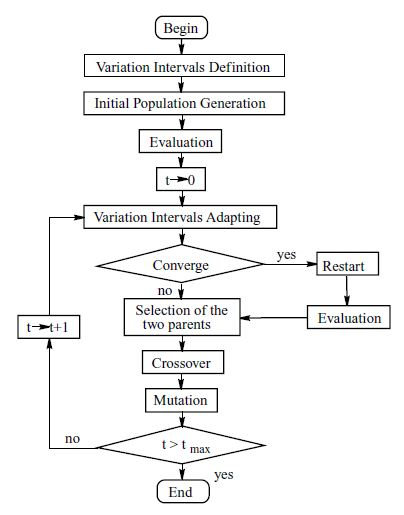
\includegraphics[width=0.45\textwidth]{imgs/flowchart-ga.JPG}
	\caption{Ddiagrama de flujo del algoritmo WMC-SSGA.}
	\label{fig:flowchart-ga}
\end{figure}

No se va a entrar en detalle con el funcionamiento del algoritmo genético, pero se podría resumir de la siguiente manera:

El WMC-SSGA comienza con la generación de una población inicial dentro de unos límites. Estas soluciones potenciales codifican parámetros para el controlador difuso, que serán evaluadas por el algoritmo basándose en una función objetivo multicriterio ponderada (con indicadores como minimizar el consumo energético y mantener los niveles de confort). Si no hay suficiente mejora, se ajustan los límites, y después, se seleccionan las mejores soluciones (padres), que se combinan y modifican para crear nuevas soluciones. Este proceso se repite de forma iterativa, evaluando y mejorando las soluciones hasta llegar a un límite o encontrar una solución lo suficientemente buena.

El método anterior contrasta con el FLC unificado, que carece de capacidades de autoajuste y depende únicamente de reglas definidas por expertos.

\subsubsection{Pruebas}

Se llevaron a cabo experimentos tanto en simulaciones como en entornos reales. Los primeros permitieron evaluar durante períodos de 10 días las distintas configuraciones del controlador bajo condiciones climáticas específicas; mientras que los segundos proporcionaron validación en condiciones más realistas. Los resultados se compararon con un controlador convencional On-Off y con versiones iniciales no optimizadas del FLC para medir la mejora alcanzada.

\subsubsection{Resultados y conclusiones}

Al igual que el controlador difuso unificado, los resultados de este estudio mostraron mejoras significativas en comparación con los controladores tradicionales.

En términos de eficiencia energética, en este estudio se lograron ahorros de hasta un 20\% en algunos casos gracias al uso de algoritmos genéticos, mientras que los parámetros de confort se mantuvieron dentro de los rangos deseados con fluctuaciones mínimas. Estos resultados sugieren que la integración de técnicas avanzadas de optimización puede potenciar aún más la eficacia de los controladores difusos.

\subsection{Sistema de inferencia difusa centrado en la evaluación de IEQ}

El sistema propuesto por Karol Jabłonski y Tomasz Grychowski, miembros de una universidad polaca, se diseñó para evaluar las condiciones ambientales interiores en un edificio mediante un sistema de sensores y un módulo de inferencia difusa. Similar al controlador difuso unificado, este sistema se enfocó en múltiples parámetros como temperatura, humedad y CO2, pero también integró otros factores como iluminación, ruido y olores, proporcionando una evaluación más completa del confort interior \parencite{jablonski2018fuzzy}.

\subsubsection{Diseño del controlador difuso}

Este estudio adoptó un sistema híbrido de inferencia difusa para procesar múltiples índices, utilizando una estructura modular con subsistemas independientes para manejar los distintos parámetros.

La \autoref{fig:fuzzy-inference-system-diagram} representa el funcionamiento del sistema de inferencia difusa, que se distingue por su enfoque integral, al combinar múltiples parámetros ambientales mediante subsistemas especializados que contribuyen a una evaluación global del confort. 

Las variables monitoreadas incluyen temperatura del aire, temperatura de globo negro, humedad relativa, densidad de CO2, iluminación, ruido y olores, que se procesan a través de módulos de inferencia difusa para estimar diferentes índices de confort. Cada uno de estos índices (confort térmico, frescura del aire y fatiga) es calculado de forma independiente y luego integrado en un módulo principal que genera una evaluación global del confort percibido.

Así, a diferencia de los otros dos sistemas que se centran en un conjunto más reducido de variables, este enfoque incluye factores adicionales como olores y ruido, que pueden tener un impacto significativo en la percepción del confort.

\begin{figure}[H]
	\centering
	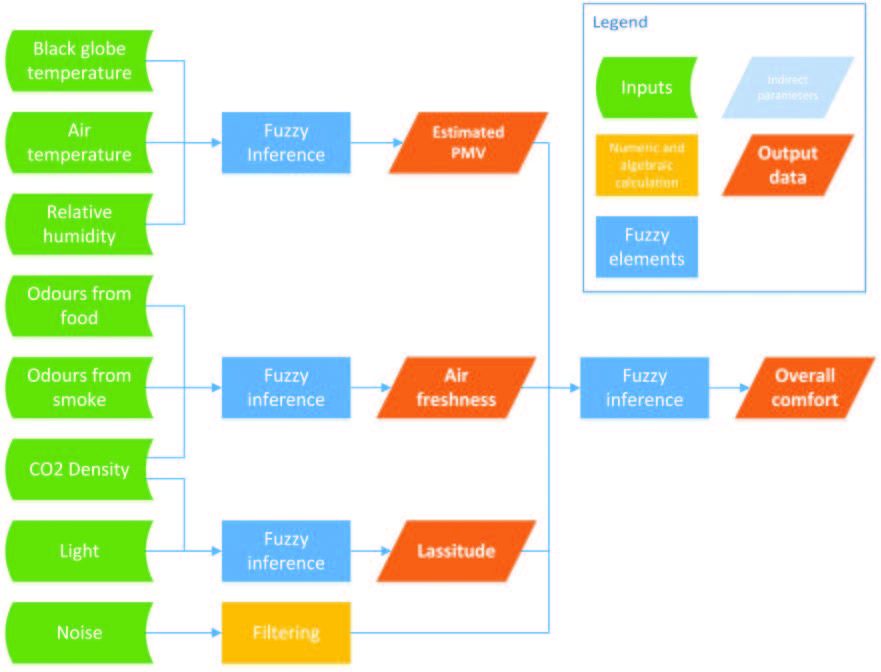
\includegraphics[width=0.7\textwidth]{imgs/fuzzy-inference-system-diagram.JPG}
	\caption{Diagrama del sistema de inferencia difusa}
	\label{fig:fuzzy-inference-system-diagram}
\end{figure}

 

Además, este sistema destaca por implementar un módulo de inferencia en \textit{LabVIEW}, diseñando desde cero los bloques de fuzzificación, inferencia y desfuzzificación, mientras que en otros estudios se utilizaron herramientas estándar o adaptaciones de controladores PID.

\subsubsection{Pruebas}

Las pruebas en este sistema se realizaron en un entorno real, con mediciones de confort en diferentes condiciones, incluyendo variaciones en ocupación y ventilación en múltiples escenarios. 

Durante las pruebas, se realizaron encuestas para validar los índices calculados por el sistema, permitiendo alinear las percepciones humanas con las salidas del sistema y obteniendo una alta concordancia entre ambas. El enfoque anterior no está presente en los otros dos estudios, donde la validación se centró más en la comparación con sistemas tradicionales o en el análisis de la eficiencia energética.

\subsubsection{Resultados y conclusiones}

Al igual que los sistemas mencionados anteriormente, este demostró una capacidad efectiva para mantener condiciones óptimas de confort interior. Además, destacó por la detección de eventos específicos como la presencia de alimentos o cambios en la ocupación. De esta forma, este sistema amplía el rango de variables monitoreadas y evaluadas, proporcionando una evaluación más centrada en todo aquello que define IEQ.

\subsection{Comparaciones entre los tres estudios}

Las comparaciones entre FLCs diseñados se han realizado en base a cinco aspectos generales:

\begin{table}[H]
	\centering
	\renewcommand{\arraystretch}{1.5}
	\begin{tabular}{|p{2.5cm}|p{4.1cm}|p{4.1cm}|p{4.1cm}|}
		\hline
		\rowcolor{lightgray}
		\textbf{Aspecto} & \textbf{Controlador difuso unificado} & \textbf{Controlador con algoritmos genéticos} & \textbf{Sistema de Inferencia Difusa} \\ \hline
		
		\textbf{Variables controladas} & 
		Temperatura, humedad, CO2, iluminación & 
		Temperatura, humedad, con optimización dinámica & 
		Temperatura, humedad, CO2, iluminación, ruido, olores \\ \hline
		
		\textbf{Enfoque metodológico} & 
		Controlador difuso clásico con reglas definidas por expertos. FLC supervisa PIDs para HVAC & 
		Integración de algoritmos genéticos para optimizar automáticamente reglas y funciones de membresía & 
		Arquitectura modular con subsistemas independientes. Implementación en LabVIEW \\ \hline
		
		\textbf{Pruebas y validación} & 
		Pruebas en una habitación piloto controlada, comparando con controlador reactivo & 
		Simulaciones y pruebas en múltiples entornos reales bajo diferentes condiciones estacionales & 
		Pruebas en entornos ocupados reales, correlacionando resultados con encuestas de usuarios \\ \hline
		
		\textbf{Objetivo principal} & 
		Optimizar el confort interior y la eficiencia energética en sistemas HVAC & 
		Equilibrio dinámico entre confort y eficiencia energética & 
		Evaluación integral del confort interior basado en múltiples índices \\ \hline
		
		\textbf{Aplicación recomendada} & 
		Escenarios con reglas de confort bien definidas, simplicidad y robustez & 
		Entornos donde se requiere máxima eficiencia energética y adaptabilidad & 
		Edificios donde la percepción humana del confort es crítica \\ \hline
	\end{tabular}
	\caption{Comparación de tres estudios sobre controladores difusos para IEQ.}
	\label{tab:comparacion}
\end{table}

En conjunto, estos tres enfoques destacan la flexibilidad de los controladores difusos y su capacidad para adaptarse a distintas necesidades y restricciones operativas.

La elección entre estos enfoques dependerá del contexto de aplicación y los objetivos específicos, como si se busca mayor integración en sistemas existentes o una evaluación más detallada de los parámetros de confort.